\documentclass[11pt]{article}
\usepackage[polish]{babel}
\usepackage[T1]{fontenc}
\usepackage[utf8]{inputenc}
\usepackage{graphicx}

\begin{document}

\begin{huge}
\begin{center}
\textbf{Automat komórkowy w języku C}\\
\end{center}
\end{huge}

\section{Wstęp}
Automat komórkowy jest systemem składającym się z pojedynczych komórek sąsiadujących ze sobą. Każda komórka przyjmuje jeden ze skończonego zbioru stanów. Komórka zmienia swój stan na podstawie przyjętych założeń, opierających się na stanie komórek z nią sąsiadujących. Takim przykładem automatu komórkowego jest gra w życie. Jej zasady to:
Jeśli żywa komórka ma 2 lub 3 żywych sąsiadów to pozostaje żywa, w przeciwnym wypadku umiera. Jeśli martwa komórka ma 3 żywych sąsiadów to ozywa, inaczej pozostaje martwa.
W naszej grze wykorzystywane jest sąsiedztwo Moore’a, które zakłada sąsiedztwo 8 komórek wokół komórki badanej.


\section{Kompilacja kodu oraz wywołanie programu}

W naszym projekcie przyjęliśmy, że przy wywoływaniu programu podawany jest plik o przykładowym wyglądzie: 
\\
3 4 
\\
1 0 0
\\
1 1 1
\\
1 1 1
\\
0 0 0
\\
W pierwszym wierszu pliku mamy wymiary planszy. Liczba 3 jest liczbą kolumn, natomiast liczby 4 jest liczbą wierszy naszej tablicy. Następne wiersze to już sama plansza, w której 0 reprezentują komórki martwe, a 1 komórki żywe.Aby wywołać program otwieramy terminal, a następnie wchodzimy w folder, w którym program się znajduje. Do terminalu wpisujemy komendę \textit{make}, która korzystając z reguł zawartych w pliku Makefile kompiluje nasz kod oraz tworzy program $GameofLife$.Następnie wywołujemy program z wybranym przez nas plikiem, np.\\
$./GameofLife$ $twojplikzdanymi.txt.$
\\
Program przechowuje planszę w tablicy dwuwymiarowej. Tworzone są 2 tablice. Jedna z nich używana jest do wprowadzania zmian w generacji, a druga służy do porównywania sąsiedztwa komórki w celu wprowadzenia zmian w pierwszej tablicy.

\section{Funkcjonowanie programu}
Program podzielono na dwa pliki $main.c$ i $funkcje.c$ oraz na plik nagłówkowy $funkcje.h$. Pierwszy z plików odpowiada za otwarcie pliku oraz wywołanie funkcji zawartych w drugim pliku.
Kolejne etapy działania programu:
\\
1.	Pobranie danych z pliku i zapisanie ich do tablic.
\\
2.	Spytanie o ilość generacji i zapisanie tej danej.
\\
3.	Wygenerowanie nazwy pliku do generacji.
\\
4.	Porównanie komórek i wygenerowanie nowej planszy.
\\
5.  Utworzenie pliku *.png z wygenerowaną uprzednio nazwą i zapisanie do niego planszy w postaci komórka żywa - kolor biały, komórka martwa - kolor czarny.
\\
Plik Makefile, o którym była mowa wcześniej zawiera 2 reguły, które kompilują kod zawarty w w plikach main.c oraz funkcje.c z flagą -lpng, aby dołączyć bibliotekę libpng. Korzystamy również z utworzonego przez nas pliku nagłówkowego "funkcje.h".
\\
Wynikiem działania programu są pliki nazwie Gen[x].png , gdzie x jest numerem generacji.

\section{Testy}
Na początku przechodzimy do folderu $Version_1.0$, w którym znajduje się nasz program. W terminal wprowadzamy komendę $make$, która pozwoli przekompilować program. Program wywoływany jest za pomocą: $GameofLife$, dodatkowo należy po $./GameofLife$ dodać nazwę pliku, na podstawie którego mają być generowane plansze. Nie podanie pliku lub podanie pliku, który nie istnieje spowoduje błąd i nasz program zakończy pracę. Jeśli program wywołamy prawidłowo spyta on nas ile planszy chcemy wygenerować.

\begin{figure}[h!]
	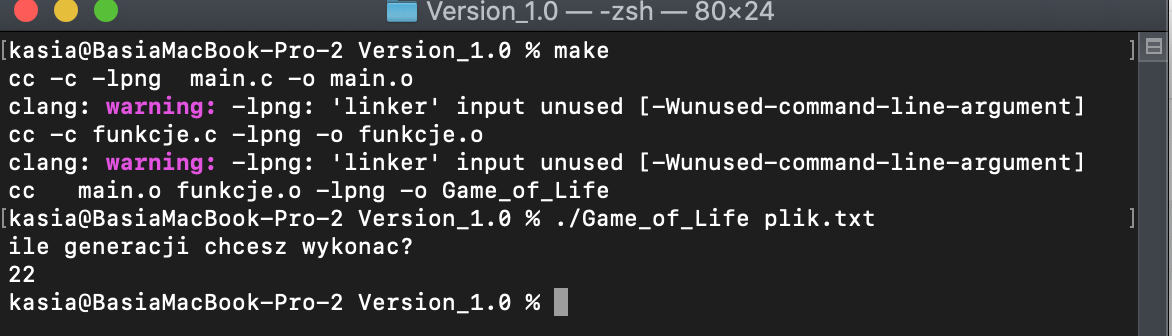
\includegraphics[width=\linewidth]{wywolanie.png}
	\caption{użycie $make$ i wywoływanie programu}
\end{figure}

\newpage Możemy potem łatwo zobaczyć, że program wygenerował pliki (w tym przykładzie 22). Dodatkowo na $Rysunku 2$ widać pliki z rozszerzeniem $*.o$, które stworzył $Makefile$.\\
\begin{figure}[h!]
	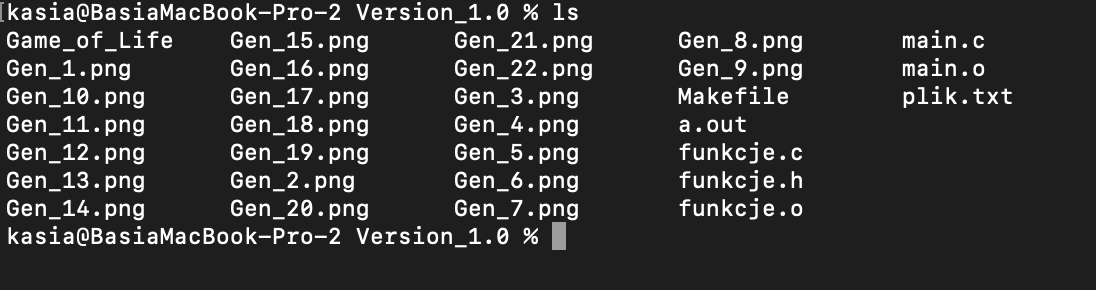
\includegraphics[width=\linewidth]{nowe_pliki.png}
	\caption{utworzone pliki}
	
	\end{figure}

Na koniec możemy wyczyścić nasz folder z wygenerowanych plansz i plików wykonywalnych ($*.o$) za pomocą komendy $make$ $clean$.

\begin{figure}[h!]
	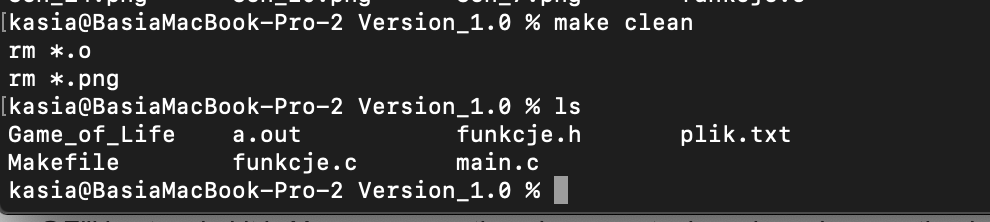
\includegraphics[width=\linewidth]{clean.png}
	\caption{$make$ $clean$}
	\end{figure}
\newpage	
\section{Pliki png}

\begin{figure}[h!]
	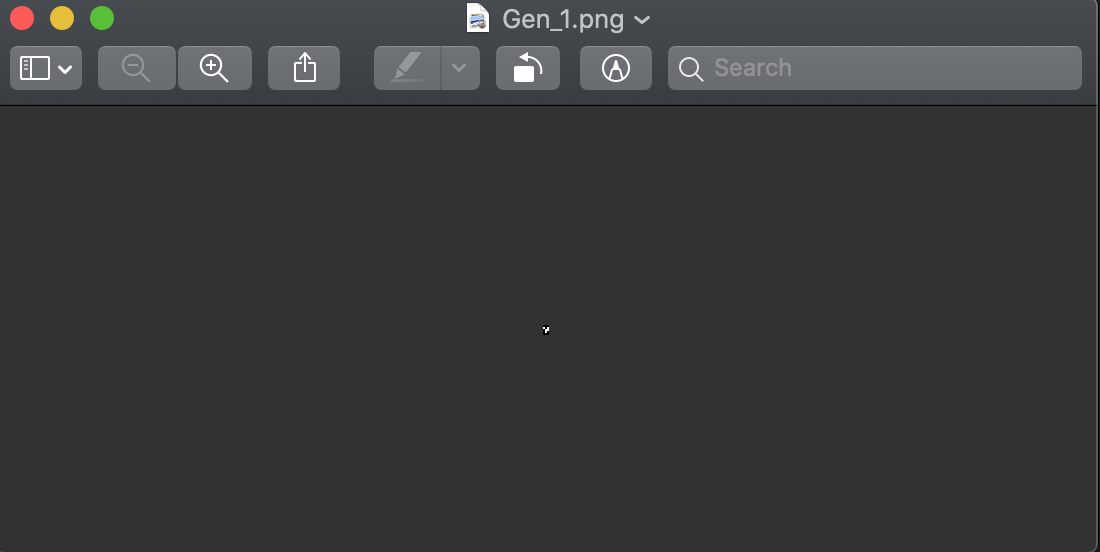
\includegraphics[width=\linewidth]{png.png}
	\caption{plik $png$}
	\label{fig:png1}
\end{figure}
Na Rysunku 4 można zauważyć, że wygenerowany plik $png$ jest bardzo mały, z tego względu trzeba oglądać go w powiększeniu (Rysunek 5).\\
\begin{figure}[h!]
	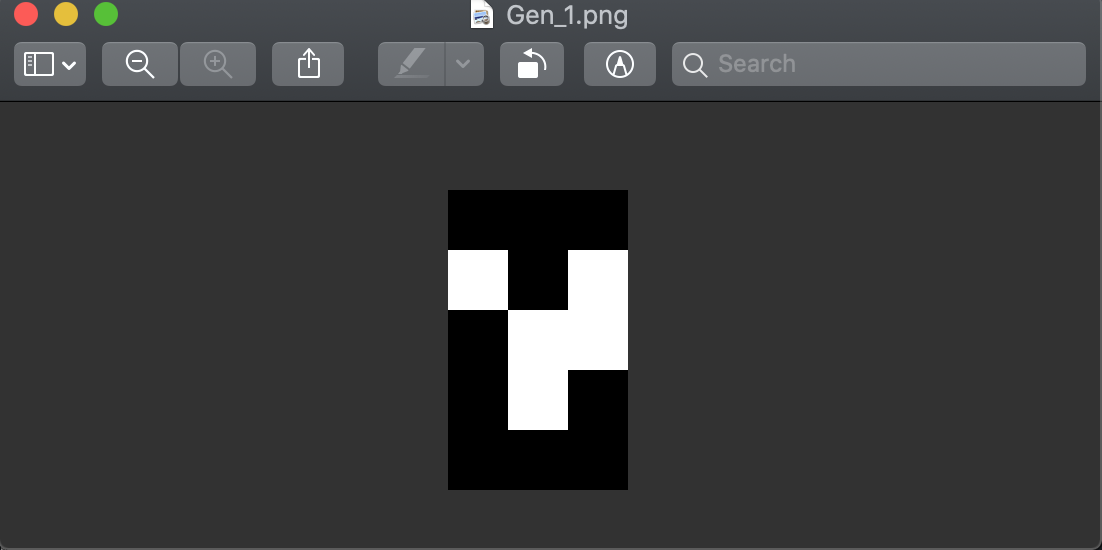
\includegraphics[width=\linewidth]{powiekszenie.png}
	\caption{Plik $png$ w powiększeniu}
\end{figure}


\section{Napotkane problemy}
Trudności w projekcie można było podzielić na dwie części: programistyczne i środowiskowe. Pierwsze dotyczyły samego napisania kodu wykonującego schemat gry w życie i dający wynik w formacie $*.png$. Drugie natomiast miały związek z obsługą Githuba, wyborem środowiska programistycznego, instalacją i konfiguracją LaTeXa. Istotą trudności projektu według mnie nie była część programistyczna, ponieważ tutaj mieliśmy już potrzebne narzędzia i tylko musieliśmy ich użyć. Natomiast druga część wymagała od nas odrobiny samodzielności i umiejętności radzenia sobie z nowymi przeszkodami.



\end{document}